%\documentclass{article}
%\documentclass[draft]{report}%{article}
\documentclass{report}%{article}
\usepackage{graphicx}
%\usepackage[draft]{graphicx}
\graphicspath{{figs}{notebooks}{.}}
\usepackage{hyperref}
\usepackage{amsmath}
\usepackage{amsfonts}
\usepackage{amssymb}
\usepackage[margin=1in]{geometry}
\usepackage{comment}
\usepackage{color}
\usepackage[acronym]{glossaries}
%\usepackage{alphalph} % For extended alphabetical numbering
\usepackage{appendix}

% \usepackage[%
%filename ,%
%content={no image available}
%]{draftfigure}

\makeglossaries
% \newacronym{label}{acronym}{definition}

\newacronym{LM}{LM}{Light Microscopy}
\newacronym{EM}{EM}{Electron Microscopy}
\newacronym{TEM}{TEM}{Transmission Electron Microscopy}
\newacronym{SEM}{SEM}{Scanning Electron Microscopy}
\newacronym{SPM}{SPM}{Scanning Probe Microscopy}
\newacronym{AFM}{AFM}{Atomic Force Microscopy}
\newacronym{STM}{STM}{Scanning Tunneling Microscope}

\newacronym{ET}{ET}{Electron Tomography}
\newacronym{cryo-ET}{Cryo-ET}{Cryo-Electron Tomography}
\newacronym{OPT}{OPT}{Optical Projection Tomography}
\newacronym{SXT}{STX}{Soft X-ray Tomography}
\newacronym{PAT}{PAT}{PhotoAcoustic Tomography}

\newacronym{GT}{GT}{Ground Truth}

\newacronym{DRV}{DRV}{Discrete Random Variable}

\newacronym{CC}{CC}{Cross-Correlation}
\newacronym{NCC}{NCC}{Normalized Cross-Correlation}
\newacronym{PCC}{PCC}{Pearson Correlation Coefficient}
\newacronym{AC}{AC}{Auto-Correlation}
\newacronym{NAC}{NAC}{Normalized Auto-Correlation}
\newacronym{SNR}{SNR}{Signal-to-Noise Ratio}
\newacronym{PSNR}{PSNR}{Peak \acrshort{SNR}}
\newacronym{SSNR}{SSNR}{Spectral Signal-to-Noise Ratio}
\newacronym{SRV}{SRV}{Stationary Random Variable}
\newacronym{FTDF}{FTDF}{Fourier Transform of a Discrete Function}
\newacronym{DTFT}{DTFT}{Discrete Time Fourier Transform}
\newacronym{IDTFT}{IDTFT}{Inverse Discrete Time Fourier Transform}
\newacronym{DFT}{DFT}{Discrete Fourier Transform}
\newacronym{IDFT}{IDFT}{Inverse Discrete Fourier Transform}
\newacronym{FFT}{FFT}{Fast Fourier Transform}
\newacronym{IFFT}{IFFT}{Inverse Fast Fourier Transform}
\newacronym{PS}{PS}{Power Spectrum}
\newacronym{PSD}{PSD}{Power Spectral Density}
\newacronym{CPSD}{CPSD}{Cross-Power Spectral Density}
\newacronym{MAD}{MAD}{Mean Absolute Deviation}

\newacronym{AWG}{AWG}{Additive White Gaussian}
\newacronym{PDF}{PDF}{Probability Density Function}
\newacronym{PMF}{PMF}{Probability Mass Function}
\newacronym{PMD}{PMD}{Probability Mass Distribution}
\newacronym{MPG}{MPG}{Mixed Poisson-Gaussian}

\newacronym{FSC}{FSC}{\href{https://en.wikipedia.org/wiki/Fourier_shell_correlation}
{Fourier Shell Correlation}}
\newacronym{SFRC}{SFRC}{Self Fourier Ring Correlation}
\newacronym{FRC}{FRC}{Fourier Ring Correlation}
\newacronym{FC}{FC}{Fourier Correlation}
\newacronym{SFC}{SFC}{Self Fourier Correlation}

\newacronym{DOF}{DOF}{Dense Optical Flow}
\newacronym{EOS}{EOS}{Even-Odd Splitting}
\newacronym{CBS}{CBS}{ChessBoard Splitting}
\newacronym{ICBS}{ICBS}{Interpolated \acrshort{CBS}}
\newacronym{SCBS}{SCBS}{Subsampled \acrshort{CBS}}
\newacronym{SPRS}{SPRS}{Structure Preserving Random Shuffling}
\newacronym{TRPR}{TRPR}{TriS-D Random Pixel Resampling}

\newacronym{MSE}{MSE}{Mean Square Error}
\newacronym{RMSE}{RMSE}{Root \acrshort{MSE}}
\newacronym{SSIM}{SSIM}{Structural Similarity Index Measure }
\newacronym{MS-SSIM}{MS-SSIM}{Multi-Scale \acrshort{SSIM}}
\newacronym{LPIPS}{LPIPS}{Learned Perceptual Image Patch Similarity}
\newacronym{NIQE}{NIQE}{Natural Image Quality Evaluator}
\newacronym{CS}{CS}{Cosine Similarity}

\newacronym{CLT}{CLT}{Central Limit Theorem}
\newacronym{GAT}{GAT}{Generalized Anscombe Transform}
\newacronym{VST}{VST}{Variance-Stabilizing Transform}
\newacronym{MNI}{MNI}{Mean of Noisy Instances}

\newacronym{GF}{GF}{Gaussian Filtering}
\newacronym{WF}{WF}{Wiener Filtering}
\newacronym{GD}{GD}{Gaussian Denoising}
\newacronym{TF}{TF}{Transfer Function}
\newacronym{LTI}{LTI}{Linear Time-Invariant}
\newacronym{NoO}{NoO}{Number of Operations}
\newacronym{IIR}{IIR}{Infinite Impulse Response}
\newacronym{FIR}{IIR}{Finite Impulse Response}

\newacronym{CNN}{CNN}{Convolutional Neural Network}

\newacronym{BM3D}{BM3D}{Block-Matching and 3D filtering}
\newacronym{DnCNN}{DnCNN}{Denoising \acrshort{CNN}}

\title{Denoising in Microscopy Imaging}

\author{Vicente González-Ruiz and José Jesús Fernández Rodríguez}

\begin{document}
\maketitle
\tableofcontents

\section*{Definitions and notation}
%{{{

\begin{tabular}{ll}
  $x$ & A scalar value (e.g., a value of a pixel of a grayscale image) \\
  $s(t)$ & A (continuous) signal as a function of time \\
  $s[n]$ & A discrete signal (only) defined at instants of time $tn, n\in\mathcal{Z}, t>0$ \\
  $\mathbf{s}$ & A digital (discrete and finite) signal (e.g., an image) \\
  $\mathbf{s}_{i}$ & The $i$-th element of $\mathbf{s}=\{\mathbf{s}_{i}\}_{i=0}^{N-1}=\{\mathbf{s}_{i}\}$ \\
  %$A[b]$ & The $b$-th element of the sampled version of $A(b)$ \\
  $\{i\}$ & The set $i$ \\
  $\mathbf{s}_{\{i\}}$ & The elements of $\mathbf{s}$ with indices $\{i\}$ \\
  $\mathbf{s}_{[i]}$ & A window of samples of $\mathbf{s}$ centered at the $i$-th sample \\
  $\mathbf{s}_{\href{https://numpy.org/doc/stable/user/basics.indexing.html#slicing-and-striding}{y,:}}$ & The $y$-th row of the image $\mathbf{s}$ \\
  $\mathbf{s}_{:,x}$ & The $x$-th column of the image $\mathbf{s}$ \\
  $\mathbf{s}_{y,x}$ & The pixel $(y,x)$ of the image $\mathbf{s}$ \\
  %$\mathbf{x}^{(i)}$ & The $i$-th real-noisy instance of the signal $\mathbf{x}$ \\
  %$\mathbf{s}^{()}$ & An instance of $\mathbf{s}$, possibly noisy \\
  $\mathbf{s}^{(i)}$ & The $i$-th instance of the signal $\mathbf{s}$ \\
  $\tilde{\mathbf{s}}^{(I)}$ & Approximation to $\mathbf{s}$ using $I$ instances \\ 
  $\overline{\mathbf{s}}$ & A mean of the samples of $\mathbf{s}$ \\ 
  $\href{https://docs.python.org/3/library/functions.html#len}{\text{len}}(\mathbf{s})$ & $=\mathbf{s}.\href{https://numpy.org/doc/stable/reference/generated/numpy.ndarray.size.html}{\mathsf{size}}$ Number of elements in $\mathbf{s}$ \\
  $\href{https://numpy.org/doc/stable/reference/generated/numpy.shape.html}{\text{shape}}(\mathbf{s})$ & ($=\mathbf{s}.{\mathsf{shape}}$) Shape of $\mathbf{s}$ \\
  $\text{rank}(\mathbf{s})$ & ($=\mathbf{s}.\mathsf{rank}=\text{len}(\mathbf{s}.\mathsf{shape})$) Dimensionality of $\mathbf{s}$ \\
  $\mathsf{\href{https://docs.python.org/3/library/functions.html\#func-range}{range}}(s)$ & $=\{0, 1, \cdots, s-1\}$ \\
  $\mathsf{\href{https://numpy.org/doc/stable/reference/generated/numpy.zeros_like.html}{zeros\_like}}(\mathbf{s})$ & $=\{0\}_{i=0}^{\mathbf{s}.\mathsf{size}-1}$ \\
  % $|\mathbf{X}_i|$ & The absolute value of $\mathbf{X}_i$ \\
  $\alpha\mathbf{s}$ & $=\{\alpha\mathbf{s}_i\}$ (scalar multiplication) \\
  $\mathbf{x}+\mathbf{y}$ & $=\{\mathbf{x}_i + \mathbf{y}_i\}$ (Hadamard addition) \\ 
  $\mathbf{x}\mathbf{y}$ & $=\{\mathbf{x}_i\mathbf{y}_i\}$ (Hadamard product) \\ 
  $\mathcal{N}$ & The normal distribution \\ 
  $\mathcal{P}$ & The Poisson distribution \\
  $\mathbf{x}\sim\mathcal{N}$ & The elements of $\mathbf{x}$ follows a normal distribution \\
  $\mathbf{x}_{\mathcal{N}}$ & The same as $\mathbf{x}\sim\mathcal{N}$ \\
  $\Pr(\mathbf{x}=a)$ & Probability that a $\mathbf{x}_i$ takes the value $a$ \\
  $\Pr(\mathbf{x}=a, \mathbf{y}=b)$ & $\Pr(\mathbf{x}=a)$ and $\Pr(\mathbf{y}=b)$ (joint probability)  \\
  $\text{Su}(\mathbf{x})$ & $=\{x\in\mathbb{R}|\Pr(\mathbf{x}=x)>0\}$ (support of $\mathbf{x}$)\\
  $\Pr(A|B)$ & Conditional probability of $A$ given $B$ \\
  $\mathbb{E}(\mathbf{s})$ & Expectation of $\mathbf{s}$ \\
  $\mathbb{V}(\mathbf{s})$ & Variance of $\mathbf{s}$ \\
  $||\mathbf{s}||_2$ & $L_2$ norm of $\mathbf{s}$ \\
  $f_s$ & Sampling frequency \\
  $\mathcal{F}$ & The (forward) Fourier transform ($\mathcal{F}(\mathbf{s})=\mathbf{S}$) (see Section~\ref{sec:Fourier_transform})\\
  $\mathcal{F}^{-1}$ & The inverse Fourier transform ($\mathcal{F}^{-1}(\mathbf{S})=\mathbf{s}$)  (see Section~\ref{sec:Fourier_transform})\\
  $\cdot^*$ & the complex conjugate of $\cdot$ \\
  $\mathbf{x}*\mathbf{y}$ & $=\mathcal{F}^{-1}(\mathcal{F}(\mathbf{x})\mathcal{F}(\mathbf{y}))=\mathcal{F}^{-1}(\mathbf{X}\mathbf{Y})$ (convolution) \\
  $A(b)$ & $A$ depends on (parameter) $b$ \\
  $A.b$ & The $b$ component of the data structure $A$ \\
  $(A)b$ & First $A$, then $b$ \\
  $E(\mathbf{s})$ & Energy of $\mathbf{s}$ (see Section~\ref{sec:energy_signal}) \\
  $P(\mathbf{s})$ & Power of $\mathbf{s}$ (see Section~\ref{sec:power_signal}) \\
  $\text{PS}(\mathbf{s})$ & Power spectrum of $\mathbf{s}$ (see Section~\ref{sec:power_spectrum}) \\
  $\text{PSD}(\mathbf{s})$ & Power spectral density of $\mathbf{s}$ (see Section~\ref{sec:PSD}) \\
  $\text{CC}(\mathbf{x},\mathbf{y})$ & Cross-correlation between $\mathbf{x}$ and $\mathbf{y}$ (see Section~\ref{sec:cross-correlation}) \\
  $\text{NCC}(\mathbf{x},\mathbf{y})$ & Normalized cross-correlation between $\mathbf{x}$ and $\mathbf{y}$ (see Section~\ref{sec:cross-correlation}) \\
  $\mathbf{a}\bot \mathbf{b}$ & $\mathbf{a}$ and $\mathbf{b}$ are orthogonal or independent                                
\end{tabular}

%}}}

\chapter{Image acquisition}
% Medical Image Acquisition

With the exception of nuclear medicine\footnote{In nuclear medicine
  imaging, radioactive substances are injected or ingested, and it is
  the physiological interactions of the agent that give rise to the
  information in the images \cite{bushberg2011essential}.}, all
medical imaging techniques require that the energy used to penetrate
the body’s tissues also interacts with those tissues.\footnote{If
  energy were to pass through the body and not experience some type of
  interaction (e.g., absorption or scattering), then the detected
  energy would not contain any useful information regarding the
  internal anatomy, and thus it would not be possible to construct an
  image of the anatomy using that information
  \cite{bushberg2011essential}.}

The power, energy and time required to acquiring medical images
require a compromise between patient safety and image
quality.\footnote{Better x-ray images can be made when the radiation
  dose to the patient is high, better magnetic resonance images can be
  made when the image acquisition time is long, and better ultrasound
  images result when the ultrasound power levels are large
  \cite{bushberg2011essential}.}


\section{Ultrasound imaging}

\chapter{Storage}
\part{Medical Images Storage}

\chapter{Basic concepts}

\section{Storage media charactaristics}
\begin{enumerate}
\item \textbf{Capacity}: This is the total amount of data that a
  storage medium can hold. It's typically measured in \popup{B}{byte}s
  (8 \popup{bits, where a bit represents a logical state with one of
    two possible values.}), \popup{KB}{kilobyte}s
  ($1\text{KB} = 2^{10}\text{B}$), \popup{MB}{megabytes}s
  ($1\text{MB} = 2^{10}\text{KB}$), \popup{GB}{gigabyte}s
  ($1\text{GB} = 2^{10}\text{MB}$), \popup{TB}{terabyte}s
  ($1\text{TB} = 2^{10}\text{GB}$), and \popup{PB}{petabyte}s
  ($1\text{PB} = 2^{10}\text{GB}$).
\item \textbf{Volatility}: If the media need to connected to a current supply (for example, the \gls{RAM} memory of a computer), the media is said \emph{volatile}.
\item \textbf{\gls{WORM}}: A \gls{CDROM}, for example.
\end{enumerate}
\begin{itemize}
\item There are many storage media capable of storing digital images (some allow
\begin{enumerate}
\item 
\item Common massive storage systems (not only used for medical images) are:
\begin{enumerate}
\item \textbf{Cloud Storage} (Google Drive, Microsoft One Drive,
etc.): data is stored in remote servers accessed over the Internet.
\item \textbf{NAS (Network-Attached Storage)}: data is stored in a
\popup{specialized computer}{The computer rarely has a keyboard or
monitor, and has many hard drive bays.} (connected to the
\popup{LAN}{Local Area Network.}) that usually mounts several disks
with some type of \popup{RAID}{Redundant Array of Independent Disks.}
configuration.
\end{enumerate}
\end{itemize}
\vspace{-4ex}
\begin{figure}[!b]
  \centering
  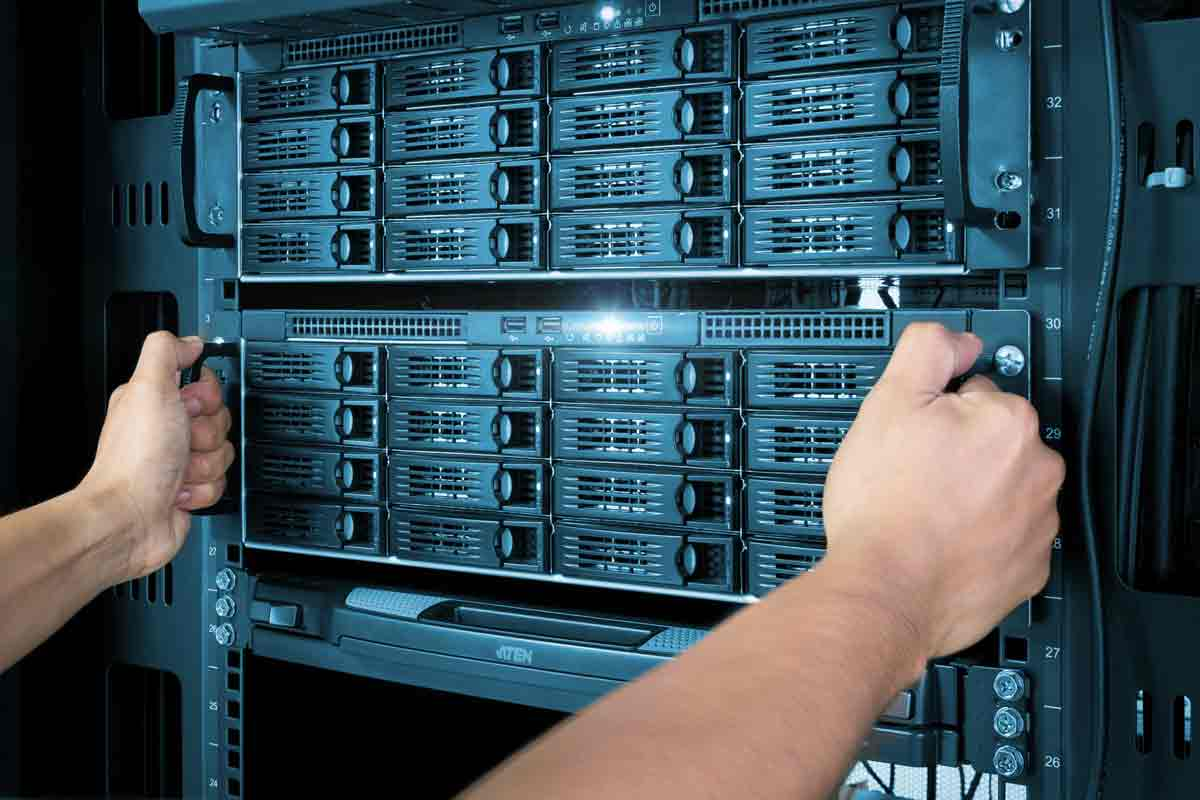
\includegraphics[height=3.5cm]{servidor-nas}
  \caption{A NAS \cite{AURUM_NAS}.\label{fig:NAS}}
\end{figure}

\section{Arrays of redundant disks}
\begin{itemize}
\item A \gls{RAID} is a logical disk that is able to work even when some of the \popup{physical disks}{That actually store the data.} fail. These are some of the existing configurations:
  \begin{enumerate}
  \item RAID-0 (Striping): \popup{No redundancy}{To maximize capacity,
      splits data across drives. This means that if a physical disk
      stops working, a loss of data will happen.}.
  \item RAID-1 (Mirroring): \popup{Maximum redundancy}{All physical
      disks contain the same data. To lost data all disks must fail at
      the same time.}.
  \item RAID-5 (Striping with Parity): \popup{One disk
      redundancy}{This configuration can only tolerate the failure of
      one disk.}. When the broken disk is replaced, the RAID must rebuild the parity information. During this time, no other disk can fail.
  \item RAID-6 (Double Parity): \popup{Two disks
      redundancy}{Tolerate the failure of
      two disks at the same time.}.
  \end{enumerate}
\end{itemize}

\section{Files and streams}
\begin{itemize}
\item A \popup{file}{Also known as ''archive''.} is a collection of data \popup{stored}{Files are
persistent: once written, they stay there until deleted.} on a storage
medium (for example, a NAS) with a defined structure and a
name. Example: a DICOM file.
\item A stream is a continuous flow of data that is transmitted and
processed in real-time, often without being stored
permanently. Example: a videcon between a patient and a doctor.
\item Files can be \popup{accesed randomly}{We can move over the file
to read or modify a part of it.}. Streams cannot (only are accesed
sequentially).
\end{itemize}

\section{Formats}
\begin{itemize}
\item Files and streams must follow some predefined structure and
encodings that indicate how to recover the information contained.
\item Most of the image formats used in medicine follow some standard
which define they, such as for example, the DICOM format.
\end{itemize}

\section{Data compression}
\begin{itemize}
\item Images requires large amounts of data to be represented. Data
compression define the objective of an efficient encoding system:
reduce the lendth of files and streams.
\item Data compressors can be:
\begin{enumerate}
\item \textbf{Lossless}: If after the decompression we recover all the
compressed information, to the point that the original file/stream can
be regenerated.
\item \textbf{Lossy}: when not. The advantage is that the compression
ratios are much higher, and sometimes the loss can be aceptable.
\end{enumerate}
\end{itemize}

\section{PACS (Picture Archiving and Communication System)}

The hospital system used to store, retrieve, and display medical images.

Replaces old physical films with digital archives.

Typically linked to the Electronic Health Record (EHR) so patient information and images are synchronized.

\section{long-term persistency, Data Sequrity and Privacy}
Patient images are protected health information (PHI).

Systems must follow laws like HIPAA (USA) or GDPR (Europe) for confidentiality.

Images should only be accessed by authorized healthcare professionals.
\section{PNG}
\section{JPEG}
\section{JPEG2000}
\section{DICOM}

\chapter{Transmission}
\chapter{Basic concepts}

\section{Communication link characteristics}
\begin{itemize}
\item \textbf{Capacity}: This is the total amount of data that a
  data link can transmit per second (bit-rate). It's typically measured in:
  \begin{tabular}{r|l}
    Acronym & Capacity in bits/second\\
    \hline
    1 Kbps & $10^3$\\
    1 Mbps & $10^3$ Kbps\\
    1 Gbps & $10^3$ Mbps\\
    1 Tbps & $10^3$ Gbps
  \end{tabular}
\item \textbf{Reliability}: Wired networks are more reliable
(have less \popup{\gls{BER}}{Ratio of the number of bits received in
error to the total number of bits transmitted over a specific time
interval.}) than wireless networks.
\item \textbf{Security}: Wired networks are more secure than wireless
networks.
\end{itemize}

\section{Networks, links, and channels}
\begin{itemize}
\item A \textbf{channel} is a available transmission capacity in a communication link.
\item A \textbf{link} is a point-to-point (wired) or multipoint
(wireless) physical medium that is able to transmit data. A link can have several channels.
\item A \textbf{network} is a collection of links and devices to
interconnect them (usually routers).
\end{itemize}

\section{Internet and internet}
\begin{itemize}
\item A \textbf{internet} is a network of networks.
\item \textbf{Internet} is the network of networks that we use every day.
\end{itemize}

\section{Web and web}
\begin{itemize}
\item A \textbf{web} is a communication system based on the
server/client model that use the \gls{HTTP} protocol.
\item The \textbf{Web} is the communication system (called \gls{WWW})
that runs at \popup{the Internet level}{You can run a local web at
home, only for your eyes.}. \gls{WWW} and Web are synonyms.
\end{itemize}

\section{Communication protocols}
\begin{itemize}
\item Define the steps and timmings that two (or more) networked
entities must use to communicate.
\item In the Internet, the name of the protocol \popup{suite}{There
are several protocols.} is \acrshort{TCP}/\acrshort{IP}.
\item For real-time transmissions, the suite also defines the
\gls{UDP}.
\item \gls{HTTP} is the protocol used in the Web (and any web).
\end{itemize}

\section{Packets}
\begin{itemize}
\item At the sender side, the data are splitted into packets.
\item Most of the links are \popup{multiplexed in time}{In an instant
of time, all the capacity of the link is used to transmit a packet.}.
\item Packets have two different parts:
\begin{enumerate}
\item A \textbf{header} that stores information for the \popup{correct
delivery}{Depending on the protocolo, even to solve the transmission
errors.}.
\item A \textbf{payload} that contains the data to transmit.
\end{enumerate}
\end{itemize}
\section{TCP/IP}
\section{WWW}

\chapter{Visualization and processing}
\chapter{Visualization}
Medical image visualization encompasses the entire process of displaying and presenting medical images and related information to facilitate diagnosis and clinical decision-making. It's a multidisciplinary field drawing on science and engineering, including computer sciences, medical physics, and perceptual psychology

Visualization should allow a physician to the interpret the images for accurate diagnosis

Contrast Resolution: This is the ability to detect very subtle changes in grayscale and distinguish them from image noise. It's primarily characterized by the signal-to-noise ratio (SNR) in an image

Quantum noise is common in X-ray or gamma ray images because relatively few quanta are used to limit patient radiation dose

Display should be calibrated.

The human eye perceives brightness differences non-linearly.

At low luminance, the eye is very sensitive → small changes in brightness are perceptually big.

At high luminance, the eye is less sensitive → bigger brightness jumps are needed to recognize a change in the luminance.

Luminance is measured with a photometer

The Barten model of human visual contrast sensitivity


\href{https://en.wikipedia.org/wiki/Stereoscopy}{Stereoscopy using a single image}.
\section{Multiresolution}
\section{Progressiveness}
\section{Denoising}
\section{Sharping}
\section{Contrast control}
\section{Tomography}
Voxelization: Place each pixel from the slices into a 3D voxel array according to its recorded position. Used in 3D ultrasound imaging.
\section{Interpolation}
\section{Segmentation}
\chapter{Segmentation}

\section{Where?}
\begin{itemize}
\item Used in the identifcation anatomical structures, lesions, or regions of interest.
\item Example: 3D surface reconstruction (ultrasound).
\end{itemize}
  
\section{Types of segementation}

\begin{itemize}
\item \textbf{Semantic}: Find objects inside an image and classify them according to predetermined categories.
\item \textbf{Instance}: Distinguish amount the object of the same category.
\item \textbf{Panoptic}: A particular case of instance segmentation where all the pixels of the image are classified.
\end{itemize}

\begin{figure}[H]
  \vspace{-0ex}
  \centering
  \href{https://www.labellerr.com/blog/semantic-vs-instance-vs-panoptic-which-image-segmentation-technique-to-choose/}{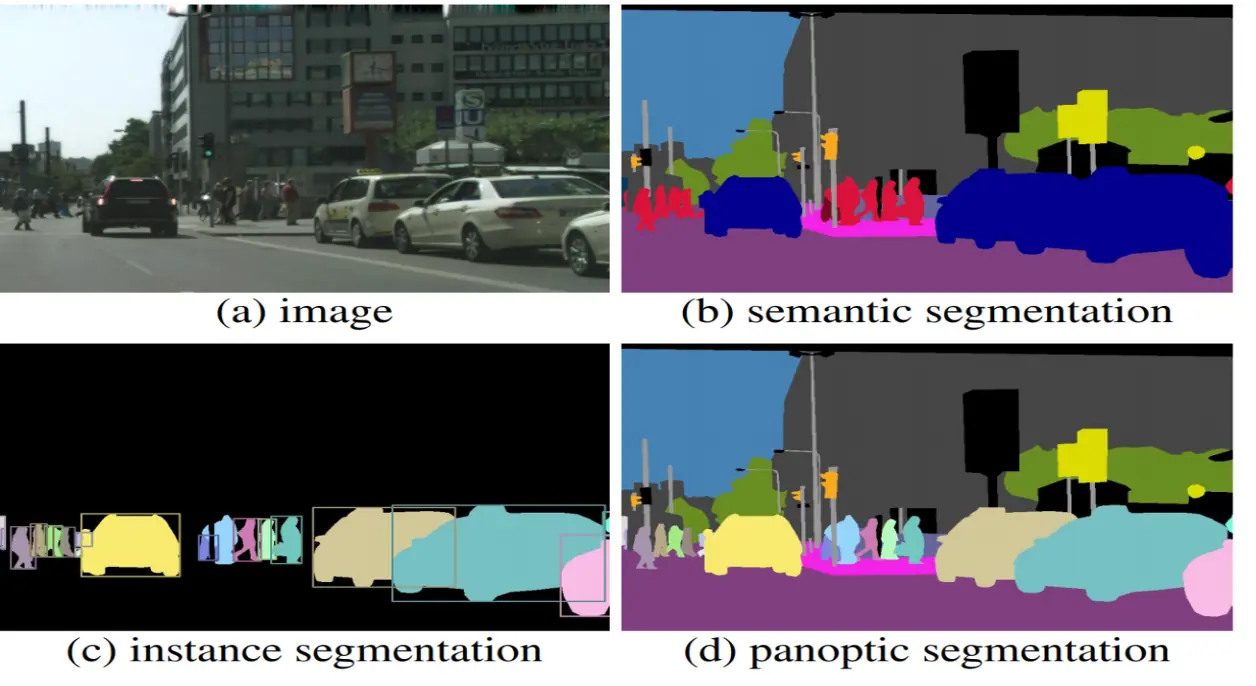
\includegraphics[width=0.9\textwidth]{semantic_vs_instance_vs_panoptic}}
  \caption{Types of segmentation.}
  \label{fig:types_segmentation}
\end{figure}

\section{Thresholding \cite{gonzalez2009digital}}
\begin{itemize}
\item Decide the classification by comparing the $I(x,y)$ pixel values with a threshold $t$, generating the binarized image
  \begin{equation}
    O(x,y) = \begin{cases*}
      1 & {\text if}\quad $I(x,y)>t$ \\
      0 & {\text otherwise}
    \end{cases*} 
  \end{equation}
  where $O(x,y)$ are the output pixel values.
\end{itemize}

\begin{figure}[H]
  \vspace{1ex}
  \centering
\href{https://github.com/vicente-gonzalez-ruiz/medical_imaging/blob/main/notebooks/thresholding.ipynb}{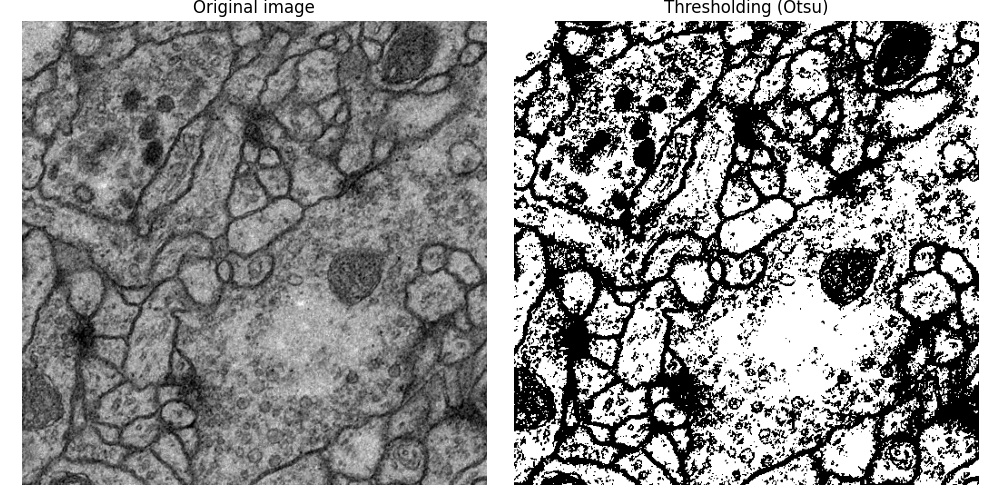
\includegraphics[width=0.9\textwidth]{thresholding}}
  \caption[An example of segmentation by thresholding.]{An example of
    segmentation by thresholding. Otsu is used for selection the
    threshold value.}
  \label{fig:thresholding}
\end{figure}

\section{U-Net segmentation \cite{ronneberger2015u}}

\begin{itemize}
\item A machine learning technique based on a deep \gls{CNN} (see Section~\ref{sec:}).
\item Supervised learning (the training set must be labeled).
\end{itemize}

%\href{https://github.com/byrkbrk/unet-implementation?tab=readme-ov-file}{unet-implementation}

%\begin{center}
%  \href{https://github.com/vicente-gonzalez-ruiz/medical_imaging/blob/main/notebooks/unet_cell_data.ipynb}{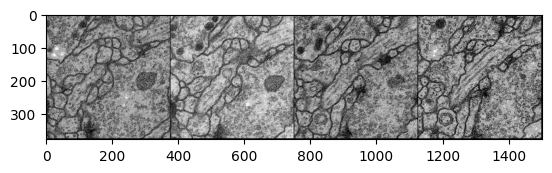
\includegraphics[width=12cm]{unet_cell_data}}
%  \href{https://github.com/vicente-gonzalez-ruiz/medical_imaging/blob/main/notebooks/unet_cell_data.ipynb}{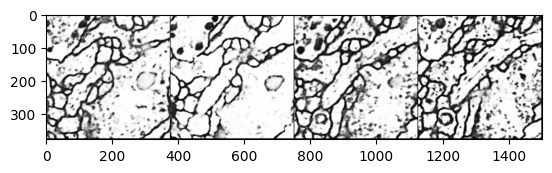
\includegraphics[width=12cm]{unet_cell_data_result}}
%\end{center}

\begin{figure}[H]
  \vspace{1ex}
  \centering
\href{https://github.com/vicente-gonzalez-ruiz/medical_imaging/blob/main/notebooks/unet_cell_data.ipynb}{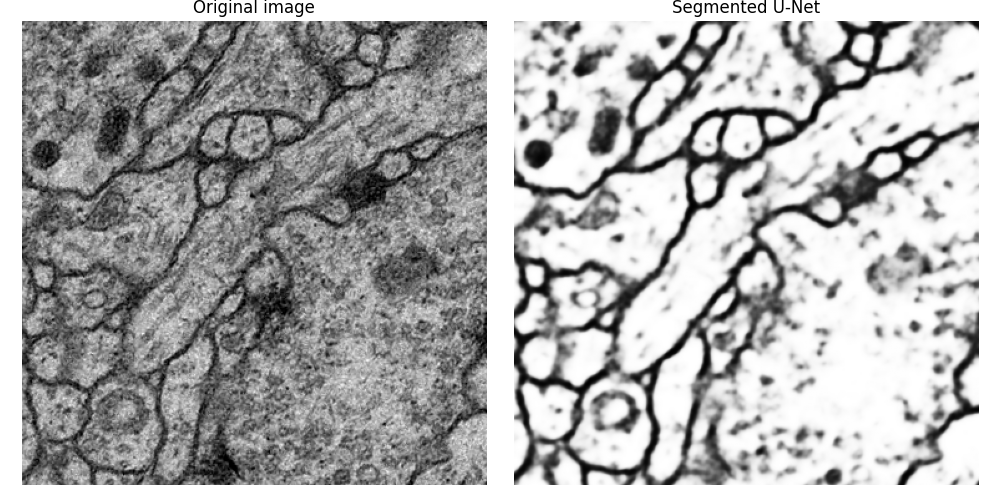
\includegraphics[width=0.9\textwidth]{U-Net_segmentation}}
  \caption[An example of segmentation using a U-Net.]{An example of
    segmentation using a U-Net. Only a crop is show.}
  \label{fig:U-Net_segmentatin}
\end{figure}



\printglossary[type=\acronymtype]

\bibliographystyle{plain}
\bibliography{tomography,MRI,denoising}

\end{document}